% MH1812 — Chapter 7: Graphs (0->100 ground-up)
\chapter[Graphs]{Graphs: Isomorphisms, Euler, Hamilton and Trees}
\label{ch:graphs}

\begin{quote}
\emph{``The bridges of K\"onigsberg are the birthplace of graph theory.''} Graphs model networks, dependencies, maps, and state spaces --- vertices and edges are enough.
\end{quote}

\noindent\fbox{\parbox{\dimexpr\linewidth-2\fboxsep-2\fboxrule}{%
\textbf{From zero: dots and lines.} A graph is just circles (vertices) joined by lines (edges). We formalise degrees, paths, cycles, then ask: when are two drawings the same graph (isomorphism)? Can we walk each edge once (Euler) or visit each vertex once (Hamilton)? What makes a tree special?}}
\vspace{0.4em}

\section*{Learning Outcomes}
After this chapter you will be able to:
\begin{enumerate}[label=(L\arabic*)]
    \item define graph, degree, path, cycle, connectivity, and graph types;
    \item test graph isomorphism via invariants and exhibit bijections;
    \item characterise Eulerian trails/circuits via parity and apply Hierholzer/K\"onigsberg;
    \item distinguish Euler vs.\ Hamilton and reason about NP-hardness intuition;
    \item characterise trees equivalently and count edges $m=n-1$.
\end{enumerate}

% ============================================================
\section{Graphs and Degrees}
\label{sec:graph-def}
A \emph{graph} $G=(V,E)$ has finite vertex set $V$ and edge set $E\subseteq\{\{u,v\}:u\neq v\}$ for simple undirected graphs. Loops and multi-edges give multigraphs; ordered pairs give digraphs. Degree $\deg(v)=|\{e:v\in e\}|$.

\begin{theorem}[Handshaking lemma]
$\sum_{v\in V}\deg(v)=2|E|$. Every edge contributes $2$ to the degree sum. Hence number of odd-degree vertices is even.
\end{theorem}

\begin{example}[Degrees]
In $K_n$ (complete graph) each $\deg=n-1$ and $|E|=\binom{n}{2}$. In $C_n$ (cycle) each $\deg=2$, $|E|=n$. In $Q_3$ (3-cube) each $\deg=3$, $|E|=12$.
\end{example}

\begin{figure}[h]\centering
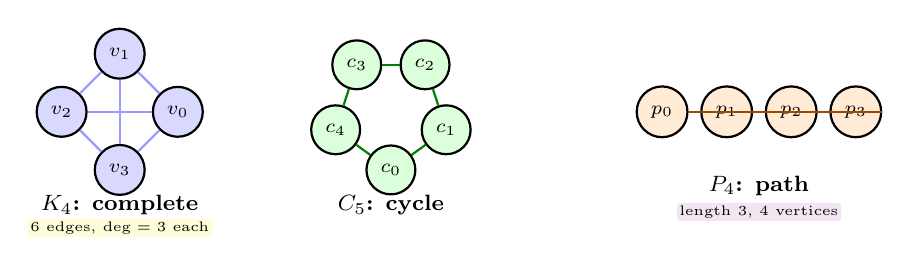
\begin{tikzpicture}[scale=0.82,every node/.style={font=\scriptsize}]
% K4, C5, and path examples with colored vertices
\begin{scope}
\foreach \i in {0,...,3} {\node[draw,circle,thick,fill=blue!15,minimum size=0.55cm] (k\i) at (90*\i:0.9) {$v_{\i}$};}
\foreach \i in {0,...,3} {\foreach \j in {0,...,3} {\ifnum\i<\j \draw[thick,blue!40] (k\i)--(k\j); \fi}}
\node[font=\footnotesize\bfseries] at (0,-1.45) {$K_4$: complete};
\node[font=\tiny,fill=yellow!15,rounded corners=1pt,inner sep=1pt] at (0,-1.80) {$6$ edges, $\deg=3$ each};
\end{scope}
\begin{scope}[xshift=4.2cm]
\foreach \i in {0,...,4} {\node[draw,circle,thick,fill=green!14,minimum size=0.55cm] (c\i) at (72*\i-90:0.9) {$c_{\i}$};}
\foreach \i in {0,...,4} {\pgfmathsetmacro{\j}{int(mod(\i+1,5))} \draw[thick,green!50!black] (c\i)--(c\j);}
\node[font=\footnotesize\bfseries] at (0,-1.45) {$C_5$: cycle};
\end{scope}
\begin{scope}[xshift=8.4cm]
\foreach \i in {0,...,3} {\node[draw,circle,thick,fill=orange!16,minimum size=0.55cm] (p\i) at (\i*1.0,0) {$p_{\i}$};}
\foreach \i in {0,...,2} {\pgfmathsetmacro{\j}{\i+1} \draw[thick,orange!60!black] (p\i)--(p\j);}
\node[font=\footnotesize\bfseries] at (1.5,-1.15) {$P_4$: path};
\node[font=\tiny,fill=violet!10,rounded corners=1pt,inner sep=1pt] at (1.5,-1.55) {length $3$, $4$ vertices};
\end{scope}
\end{tikzpicture}
\caption{Three archetypes: complete, cycle, path. Colour distinguishes families.}
\label{fig:graph-families}
\end{figure}

A \emph{path} $v_0v_1\dots v_k$ has distinct vertices (except possibly ends). A \emph{cycle} is a closed path $v_0=v_k$. $G$ is \emph{connected} if a path exists between every pair. Component = maximal connected subgraph.

\section{Isomorphism}
\label{sec:isomorphism}
$G\cong H$ if a bijection $f:V(G)\to V(H)$ preserves adjacency: $\{u,v\}\in E(G)\iff\{f(u),f(v)\}\in E(H)$. Isomorphic graphs are the same up to relabelling.

Invariants (if $G\cong H$, these match): $|V|,|E|$, degree sequence sorted, number of cycles of length $k$, connectivity, planarity. Mismatch proves non-isomorphic; matching does not prove isomorphic.

\begin{figure}[h]\centering
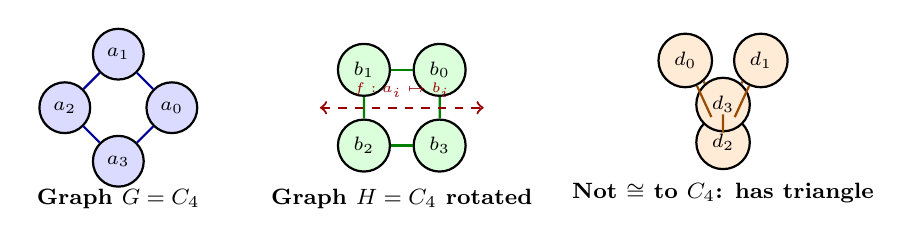
\begin{tikzpicture}[scale=0.80,every node/.style={font=\scriptsize}]
% Isomorphism example: C4 vs diamond etc.
\begin{scope}
\foreach \i in {0,...,3} {\node[draw,circle,thick,fill=blue!14,minimum size=0.55cm] (a\i) at (90*\i:0.85) {$a_{\i}$};}
\foreach \i in {0,...,3} {\pgfmathsetmacro{\j}{int(mod(\i+1,4))} \draw[thick,blue!60!black] (a\i)--(a\j);}
\node[font=\footnotesize\bfseries] at (0,-1.45) {Graph $G=C_4$};
\end{scope}
\begin{scope}[xshift=4.5cm]
\foreach \i in {0,...,3} {\node[draw,circle,thick,fill=green!14,minimum size=0.55cm] (b\i) at (90*\i+45:0.85) {$b_{\i}$};}
\foreach \i in {0,...,3} {\pgfmathsetmacro{\j}{int(mod(\i+1,4))} \draw[thick,green!50!black] (b\i)--(b\j);}
\node[font=\footnotesize\bfseries] at (0,-1.45) {Graph $H=C_4$ rotated};
\draw[<->,thick,red!60!black,dashed] (-1.3,0) -- (1.3,0) node[midway,above,font=\tiny] {$f:a_i\mapsto b_i$};
\end{scope}
\begin{scope}[xshift=9.0cm]
\foreach \i in {0,1} {\node[draw,circle,thick,fill=orange!16,minimum size=0.55cm] (d\i) at (\i*1.2,0.75) {$d_{\i}$};}
\node[draw,circle,thick,fill=orange!16,minimum size=0.55cm] (d2) at (0.6,-0.55) {$d_2$};
\node[draw,circle,thick,fill=orange!16,minimum size=0.55cm] (d3) at (0.6,0.05) {$d_3$};
\draw[thick,orange!60!black] (d0)--(d3)--(d1); \draw[thick,orange!60!black] (d0)--(d2)--(d1); \draw[thick,orange!60!black] (d2)--(d3);
\node[font=\footnotesize\bfseries] at (0.6,-1.35) {Not $\cong$ to $C_4$: has triangle};
\end{scope}
\end{tikzpicture}
\caption{Isomorphism is a relabelling that preserves edges. Invariants like ``contains a triangle'' distinguish non-isomorphic graphs.}
\label{fig:isomorphism}
\end{figure}

\begin{example}[Non-isomorphic despite same degrees]
Two $6$-vertex $3$-regular graphs exist: $K_{3,3}$ vs.\ prism. Both have $|V|=6,|E|=9$, all $\deg=3$, but one is bipartite (no odd cycle), the other has a triangle --- not isomorphic.
\end{example}

\section{Euler Trails and Circuits}
\label{sec:euler}
An \emph{Euler circuit} traverses each edge exactly once and returns to start (closed trail). An \emph{Euler trail} does so without returning.

\begin{theorem}[Euler, 1736]
A connected graph has an Euler circuit iff every vertex has even degree. It has an Euler trail (non-closed) iff exactly $0$ or $2$ vertices have odd degree ($0\to$ circuit, $2\to$ trail between the odd vertices).
\end{theorem}
\begin{proof}[Sketch] Even degrees allow pairing entry/exit at each vertex to splice cycles (Hierholzer). Odd count $\neq0,2$ makes pairing impossible.
\end{proof}

K\"onigsberg's $4$ landmasses with $7$ bridges had $4$ odd-degree vertices --- no Euler trail, hence the famous impossibility.

\begin{figure}[h]\centering
\begin{tikzpicture}[scale=0.82,every node/.style={font=\scriptsize}]
% K\"onigsberg sketch and Eulerian example
\begin{scope}
\node[draw,thick,ellipse,fill=blue!14,minimum width=1.1cm,minimum height=0.7cm] (a) at (0,0.7) {A};
\node[draw,thick,ellipse,fill=green!14,minimum width=1.1cm,minimum height=0.7cm] (b) at (0,-0.7) {B};
\node[draw,thick,ellipse,fill=orange!16,minimum width=0.9cm,minimum height=0.7cm] (c) at (-1.6,0) {C};
\node[draw,thick,ellipse,fill=violet!12,minimum width=0.9cm,minimum height=0.7cm] (d) at (1.6,0) {D};
\draw[thick,blue!60!black] (c) to[bend left=18] (a); \draw[thick,blue!60!black] (c) to[bend right=18] (a);
\draw[thick,blue!60!black] (c)--(b); \draw[thick,blue!60!black] (d)--(a); \draw[thick,blue!60!black] (d)--(b);
\draw[thick,blue!60!black] (a) to[bend left=12] (b); \draw[thick,blue!60!black] (a) to[bend right=12] (b);
\node[font=\tiny,fill=red!15,rounded corners=1pt,inner sep=1pt] at (0,-1.55) {K\"onigsberg: $4$ odd $\Rightarrow$ no Euler trail};
\end{scope}
\begin{scope}[xshift=6.2cm]
\foreach \i in {0,...,3} {\node[draw,circle,thick,fill=green!14,minimum size=0.55cm] (e\i) at (90*\i:0.85) {$v_{\i}$};}
\foreach \i in {0,...,3} {\pgfmathsetmacro{\j}{int(mod(\i+1,4))} \draw[thick,green!60!black] (e\i)--(e\j);}
\draw[thick,green!60!black] (e0)--(e2);
\node[font=\tiny,fill=yellow!15,rounded corners=1pt,inner sep=1pt] at (0,-1.45) {Euler circuit exists: all $\deg$ even};
\node[font=\tiny] at (0,-1.85) {e.g.\ $v_0\to v_1\to v_2\to v_0\to v_2\to v_3\to v_0$};
\end{scope}
\end{tikzpicture}
\caption{Left: K\"onigsberg model (multigraph). Right: a graph with all even degrees and an explicit Euler circuit.}
\label{fig:euler-konigsberg}
\end{figure}

Hierholzer's algorithm finds an Euler circuit in $O(|E|)$: walk until stuck (must be at start by even degrees), then splice in cycles from unused edges.

\section{Hamilton Cycles and Trees}
\label{sec:hamilton-trees}
A \emph{Hamilton cycle} visits each vertex exactly once and returns; a \emph{Hamilton path} visits each once. Unlike Euler (easy parity check), Hamilton is NP-complete --- no simple characterisation is known.

\begin{theorem}[Dirac]
If $n\ge3$ and every $\deg(v)\ge n/2$ then $G$ is Hamiltonian (sufficient, not necessary).
\end{theorem}

A \emph{tree} is a connected acyclic graph.

\begin{theorem}[Tree equivalences]
For $G$ with $n$ vertices, TFAE: (i) $G$ is a tree; (ii) $G$ connected and $|E|=n-1$; (iii) $G$ acyclic and $|E|=n-1$; (iv) unique path between every two vertices.
\end{theorem}
\begin{proof} (i)$\Rightarrow$(ii): induction by removing a leaf (a tree has $\ge2$ leaves). Counts telescope to $n-1$. Other implications by similar leaf/edge counting.
\end{proof}

\begin{lstlisting}[language=Python]
# Handshaking and Euler check
def has_euler_circuit(degrees): return all(d%2==0 for d in degrees)
def has_euler_trail(degrees): return sum(d%2 for d in degrees) in (0,2)
print(has_euler_circuit([2,2,2,2]), has_euler_trail([1,1,2,2]))

# Tree check: connected (BFS) + edges == n-1 and acyclic
def is_tree(n, edges):
    if len(edges)!=n-1: return False
    from collections import deque, defaultdict
    g=defaultdict(list)
    for u,v in edges:
        g[u].append(v); g[v].append(u)
    seen={0}; q=deque([0])
    while q:
        u=q.popleft()
        for w in g[u]:
            if w not in seen: seen.add(w); q.append(w)
    return len(seen)==n
print(is_tree(4, [(0,1),(1,2),(2,3)]))
\end{lstlisting}


\begin{example}[Degree sequence graphic?]
$(3,3,2,2,2)$ sums to $12=2\cdot6$, so handshaking allows it (needs $6$ edges). But $(3,3,3,1)$ sums to $10$, also even, yet no simple graph realises it (Erd\H{o}s--Gallai fails). Sum even is necessary, not sufficient.
\end{example}

\begin{theorem}[Euler's formula preview]
For connected planar graphs, $V-E+F=2$. Trees have $F=1$ (outer face), so $E=V-1$, matching the tree theorem.
\end{theorem}

\begin{remark}[Bipartite test via BFS]
$G$ bipartite iff no odd cycle (equivalently $2$-colourable). BFS $2$-colouring in $O(V+E)$ tests this --- used for $K_{3,3}$ vs.\ prism distinction.
\end{remark}

\begin{figure}[h]\centering
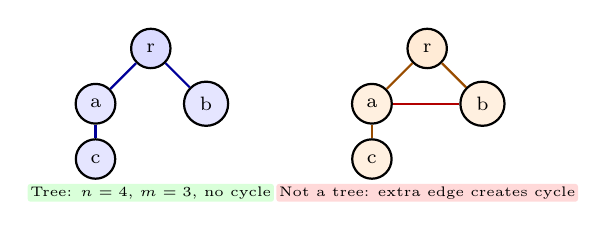
\begin{tikzpicture}[scale=0.78,every node/.style={font=\scriptsize}]
% Tree vs non-tree
\begin{scope}
\node[draw,circle,thick,fill=blue!14,minimum size=0.5cm] (t0) at (0,0.9) {r};
\node[draw,circle,thick,fill=blue!10,minimum size=0.5cm] (t1) at (-0.9,0) {a};
\node[draw,circle,thick,fill=blue!10,minimum size=0.5cm] (t2) at (0.9,0) {b};
\node[draw,circle,thick,fill=blue!10,minimum size=0.5cm] (t3) at (-0.9,-0.9) {c};
\draw[thick,blue!60!black] (t0)--(t1); \draw[thick,blue!60!black] (t0)--(t2);
\draw[thick,blue!60!black] (t1)--(t3);
\node[font=\tiny,fill=green!15,rounded corners=1pt,inner sep=1pt] at (0,-1.45) {Tree: $n=4$, $m=3$, no cycle};
\end{scope}
\begin{scope}[xshift=4.5cm]
\node[draw,circle,thick,fill=orange!16,minimum size=0.5cm] (q0) at (0,0.9) {r};
\node[draw,circle,thick,fill=orange!12,minimum size=0.5cm] (q1) at (-0.9,0) {a};
\node[draw,circle,thick,fill=orange!12,minimum size=0.5cm] (q2) at (0.9,0) {b};
\node[draw,circle,thick,fill=orange!12,minimum size=0.5cm] (q3) at (-0.9,-0.9) {c};
\draw[thick,orange!60!black] (q0)--(q1); \draw[thick,orange!60!black] (q0)--(q2);
\draw[thick,orange!60!black] (q1)--(q3); \draw[thick,red!70!black] (q1)--(q2);
\node[font=\tiny,fill=red!15,rounded corners=1pt,inner sep=1pt] at (0,-1.45) {Not a tree: extra edge creates cycle};
\end{scope}
\end{tikzpicture}
\caption{Tree vs.\ non-tree: one extra edge beyond $n-1$ forces a cycle.}
\label{fig:tree-vs-graph}
\end{figure}

Handshaking lemma is a global invariant from local degrees, a double-counting gem.
Complete graphs $K_n$ maximise edges, paths $P_n$ minimise connectivity, cycles $C_n$ sit in between.
Isomorphism is graph relabelling: invariants can disprove it, but only an explicit bijection proves it.
Degree sequence, cycle counts, and bipartiteness are quick isomorphism filters before brute force.
Euler's parity condition is a rare easy characterisation: all even degrees versus NP-hard Hamilton.

\begin{theorem}[Handshake for digraphs]
$\sum_{v}\mathrm{indeg}(v)=\sum_{v}\mathrm{outdeg}(v)=|E|$ for digraphs; the undirected version follows by splitting each undirected edge into two arcs.
\end{theorem}

\begin{example}[Bipartite vs odd cycle]
$C_3$ (triangle) is not bipartite; any graph with an odd cycle fails $2$-colouring. $K_{3,3}$ is bipartite yet non-planar (utility puzzle).
\end{example}

\subsection{Graph Colouring}
\label{sec:colouring}
A \emph{$k$-colouring} paints vertices with $k$ colours so no edge joins same-coloured endpoints; the \emph{chromatic number} $\chi(G)$ is the smallest such $k$. Intuition: colours are time slots or registers---neighbours conflict. Bipartite means exactly $\chi\le2$ (test by BFS $2$-colouring); any odd cycle forces $\chi\ge3$.
\begin{example}[Greedy bound]
Order vertices arbitrarily; paint each with the smallest colour its neighbours spare. This \emph{greedy} colouring uses at most $\Delta+1$ colours ($\Delta$ = max degree), so $\chi(G)\le\Delta+1$. On $C_5$ ($\Delta=2$) greedy meets $\chi=3$; on a star $K_{1,n}$ a bad order wastes colours a good order avoids---ordering matters.
\end{example}

\section{Worked Example: Euler vs.\\ Hamilton on the Same Graph}
Consider $C_5$ (5-cycle). All degrees $2$ even, so Euler circuit exists: walk around. Hamilton cycle also exists (the cycle itself). Now add a chord $v_0v_2$: degrees become $3,3,2,2,2$ --- two odds remain, so an Euler trail exists but not a circuit. Hamiltonian? $v_0v_1v_2v_3v_4v_0$ still works (use outer cycle). Finally $K_{2,3}$: degrees $3,3,2,2,2$ again, bipartite, Euler trail exists, Hamiltonian? $K_{2,3}$ has $5$ vertices, any Hamilton cycle needs even length to alternate parts, so none exists (part sizes differ by $1$). Invariants separate the concepts.

% ============================================================
\section{Chapter Notes}
Euler founded graph theory (1736); Hamilton's game (1857) became the TSP. Trees link to induction (leaf removal), to recursion (DFS/BFS trees), and to minimum spanning trees (SC2001). Graph isomorphism is in NP but not known to be NP-complete (Babai's quasi-polynomial).

% ============================================================
\section{Exercises}
\label{sec:ch07-exercises}
\begin{enumerate}[label=E7.\arabic*, leftmargin=*, itemsep=0.6em]
\item \textbf{Handshaking.} Prove the number of odd-degree vertices is even. Give a graph with degree sequence $(3,3,2,2,2)$ or explain why impossible.
\item \textbf{Isomorphism.} Determine if the two $4$-vertex graphs $P_4$ and $C_4$ are isomorphic via invariants. Find an explicit isomorphism between two drawn $C_4$'s or prove none exists for $C_4$ vs.\ diamond.
\item \textbf{Euler.} Which of $K_5$, $K_{3,3}$, $C_n$, $Q_3$ have Euler circuits/trails? Apply the parity theorem and, when they exist, give the trail.
\item \textbf{Hamilton vs Euler.} Give a graph with an Euler circuit but no Hamilton cycle, and one with a Hamilton cycle but no Euler circuit. Explain.
\item \textbf{Trees.} Prove a tree with $n\ge2$ has at least two leaves. Use this to prove by induction that a tree has $n-1$ edges and a unique path between any two vertices.
\end{enumerate}
% End of Chapter 7
